\documentclass{standalone}
\usepackage{tikz}
\usepackage{xinttools}

\usetikzlibrary{calc,math,intersections}


\begin{document}

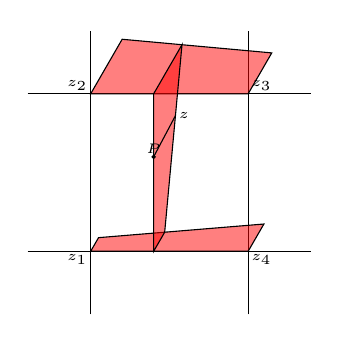
\begin{tikzpicture}[scale=2]
  \path[use as bounding box] (-0.4,-0.4) rectangle (1.4,1.42);

  \tikzmath{
    real \x;
    real \y;
    real \angle;
    \x = 0.4;
    \y = 0.6;
    \angle = 60;
  }
  \coordinate (P) at (\x,\y);
  \coordinate (P1) at (0,0);
  \coordinate (P2) at (0,1);
  \coordinate (P3) at (1,1);
  \coordinate (P4) at (1,0);

  \draw (-0.4,-0.4) grid (1.4,1.4);

  \node[anchor=north east,font=\tiny,inner sep=1pt] at (P1) {$z_1$};
  \node[anchor=south east,font=\tiny,inner sep=1pt] at (P2) {$z_2$};
  \node[anchor=south west,font=\tiny,inner sep=1pt] at (P3) {$z_3$};
  \node[anchor=north west,font=\tiny,inner sep=1pt] at (P4) {$z_4$};

  \coordinate (Q1) at ($ (0,0) + (\angle:0.1) $);
  \coordinate (Q2) at ($ (0,1) + (\angle:0.4) $);
  \coordinate (Q3) at ($ (1,1) + (\angle:0.3) $);
  \coordinate (Q4) at ($ (1,0) + (\angle:0.2) $);

  \path[opacity=0.5,fill=red] (P1) -- (Q1) -- (Q4) -- (P4) -- cycle;
  \draw (P1) -- (Q1) -- (Q4) -- (P4) -- cycle;
  \path[opacity=0.5,fill=red] (P2) -- (Q2) -- (Q3) -- (P3) -- cycle;
  \draw (P2) -- (Q2) -- (Q3) -- (P3) -- cycle;

  \path[name path=G14] (P1) -- (P4);
  \path[name path=G23] (P2) -- (P3);
  \path[name path=L14] (Q1) -- (Q4);
  \path[name path=L23] (Q2) -- (Q3);
  \path[name path=vert] (\x,0) -- (\x,2);
  \path[name intersections={of=vert and G14,by=g14},name intersections={of=vert and G23,by=g23}];
  \path[name path=V14] (g14) -- ++(\angle:1);
  \path[name path=V23] (g23) -- ++(\angle:1);

  \path[opacity=0.5,fill=red,name intersections={of=V14 and L14,by=z14},
        name intersections={of=V23 and L23,by=z23}] (g14) -- (g23) -- (z23) -- (z14) -- cycle;
  \draw[name intersections={of=V14 and L14,by=z14},
        name intersections={of=V23 and L23,by=z23}] (g14) -- (g23) -- (z23) -- (z14) -- cycle;

  \path[name path=vertP] (P) -- (\angle:2);
  \path[name path=L1234] (z14) -- (z23);
  \draw[name intersections={of=vertP and L1234,by=zz}] (P) -- (zz) node[right,inner sep=1pt,font=\tiny] {$z$};

  \draw[fill=black] (P) circle [radius=0.01cm] node[above,font=\tiny,inner sep=1pt] {$P$};
\end{tikzpicture}

\end{document}
